\section{The R\'enyi law and the duality criterion}\label{sec:renyi}

\subsection{Polynomial checks}

A check is \emph{exponential} when $r$ runs drive its false acceptance probability to $\eps^{r}$, so that the cost of reaching $\delta$ is $a\log(1/\delta)/L$. Many checks are slower. A statistical check that averages $m$ independent samples of a statistic and accepts when the average is close to its target is the basic example.

\begin{example}[Chebyshev checks]\label{ex:chebyshev}
Let a candidate determine a random variable $X$ with variance at most $\sigma^{2}$, with mean $0$ if the candidate is correct and mean at least $2t>0$ if it is incorrect, and let the check accept when the mean of $m$ independent samples is below $t$. By Chebyshev's inequality an incorrect candidate is accepted, and a correct one rejected, with probability at most $\sigma^{2}/(mt^{2})$. So false acceptance probability $\delta$ costs $m=\sigma^{2}/(t^{2}\delta)$ samples: the cost is $a\,\delta^{-1}$ with $a$ proportional to $\sigma^{2}/t^{2}$.
\end{example}

We say a family of checks has \emph{polynomial order} $s>0$ if the check of candidate $i$ reaches false acceptance probability $\delta_{i}\in(0,1]$ at cost $a_{i}\delta_{i}^{-s}$, and that an allocation $\delta$ is $\theta$-sound if $\sum_{i}\delta_{i}\le\theta$. Chebyshev checks have order $1$. Let $\Vs_{s}(\theta)$ be the infimum of $\sum_{i}a_{i}\delta_{i}^{-s}$ over $\theta$-sound allocations. For $0<\alpha<1$ the R\'enyi entropy of order $\alpha$ is
\[
H_{\alpha}(p)=\frac1{1-\alpha}\log\sum_{i}p_{i}^{\alpha},
\]
which decreases from $\log n$ at $\alpha\to0$ to $H(p)$ at $\alpha\to1$ \cite{Ren61,CT06}.

\begin{proof}[Proof of Theorem~\ref{thm:D}]
\emph{Lower bound.} Put $\alpha=1/(1+s)$, so that $1/\alpha=1+s$ and $1/(1-\alpha)=(1+s)/s$ are conjugate exponents. Write $a_{i}^{\alpha}=(a_{i}\delta_{i}^{-s})^{\alpha}\,\delta_{i}^{s\alpha}$ and apply H\"older's inequality:
\[
\begin{aligned}
\sum_{i}a_{i}^{\alpha}&\le\Bigl(\sum_{i}a_{i}\delta_{i}^{-s}\Bigr)^{\alpha}\Bigl(\sum_{i}\delta_{i}^{s\alpha/(1-\alpha)}\Bigr)^{1-\alpha}\\
&=\Bigl(\sum_{i}a_{i}\delta_{i}^{-s}\Bigr)^{\frac1{1+s}}\Bigl(\sum_{i}\delta_{i}\Bigr)^{\frac s{1+s}},
\end{aligned}
\]
since $s\alpha/(1-\alpha)=1$. With $\sum\delta_{i}\le\theta$ and raising to the power $1+s$, $(\sum_{i}a_{i}^{\alpha})^{1+s}\le\theta^{s}\sum_{i}a_{i}\delta_{i}^{-s}$.

\emph{Attainment.} Let $S=\sum_{j}a_{j}^{\alpha}$ and $\delta_{i}=\theta a_{i}^{\alpha}/S$. Then $\sum\delta_{i}=\theta$, $\delta_{i}\le\theta\le1$ because $a_{i}^{\alpha}\le S$, and $\sum_{i}a_{i}\delta_{i}^{-s}=\theta^{-s}S^{s}\sum_{i}a_{i}^{1-s\alpha}=\theta^{-s}S^{s}\sum_{i}a_{i}^{\alpha}=\theta^{-s}S^{1+s}$, because $1-s\alpha=\alpha$.

\emph{Entropy form.} $S=A^{\alpha}\sum_{i}p_{i}^{\alpha}$, so $S^{1+s}=A\,(\sum_{i}p_{i}^{\alpha})^{1+s}$, and $(1+s)\log\sum p_{i}^{\alpha}=\frac{1+s}{s}\,s\log\sum p_{i}^{\alpha}=s\,H_{\alpha}(p)$, since $1-\alpha=s/(1+s)$.

\emph{The limit $s\to0$.} For finitely many candidates $\alpha\mapsto\log\sum p_{i}^{\alpha}$ is smooth and vanishes at $\alpha=1$ with derivative $\sum p_{i}\log p_{i}=-H(p)$ there, so $H_{\alpha}(p)=H(p)+O(1-\alpha)=H(p)+O(s)$. Hence $\Vs_{s}(\theta)/A=\exp\bigl(s(H_{\alpha}(p)+\log\frac1\theta)\bigr)=1+s\bigl(H(p)+\log\frac1\theta\bigr)+O(s^{2})$.
\end{proof}

The optimal allocation gives the $i$-th check the share $a_{i}^{\alpha}/S$ of the budget, a flattened version of the share $a_{i}/A$ of the exponential case: when checks are slow, expensive checks must still be made quite reliable, because buying reliability anywhere is costly. The two laws are related by a limit. Since $\frac1L\log\frac1\delta=\lim_{s\to0}\frac{\delta^{-s}-1}{sL}$, the cost of an exponential check is the derivative at $s=0$ of the cost of a polynomial one, and
\[
\lim_{s\to0}\frac{\Vs_{s}(\theta)-A}{sL}=\frac AL\Bigl(H(p)+\log\frac1\theta\Bigr),
\]
which is the real relaxation of the entropy law (Proposition~\ref{prop:shape}). Campbell's coding theorem has the same structure, with exponentially weighted codeword lengths and the R\'enyi entropy of order $1/(1+t)$ \cite{Cam65}.

\begin{corollary}[Equal costs]\label{cor:polyuniform}
For $n$ candidates of cost $a$ and checks of order $s$, $\Vs_{s}(\theta)=a\,n^{1+s}\theta^{-s}$. Chebyshev checks cost $an^{2}/\theta$, against $(an/L)\log(n/\theta)+O(an)$ for exponential checks.
\end{corollary}

So the tax per candidate is $(n/\theta)^{s}$ for polynomial checks and $\log(n/\theta)/L$ for exponential ones: a statistical check that is not amplified exponentially makes the certification of a long run of modifications quadratically expensive. Figure~\ref{fig:renyi} shows the law and its tangent at $s=0$.

\begin{figure*}[t]
\centering
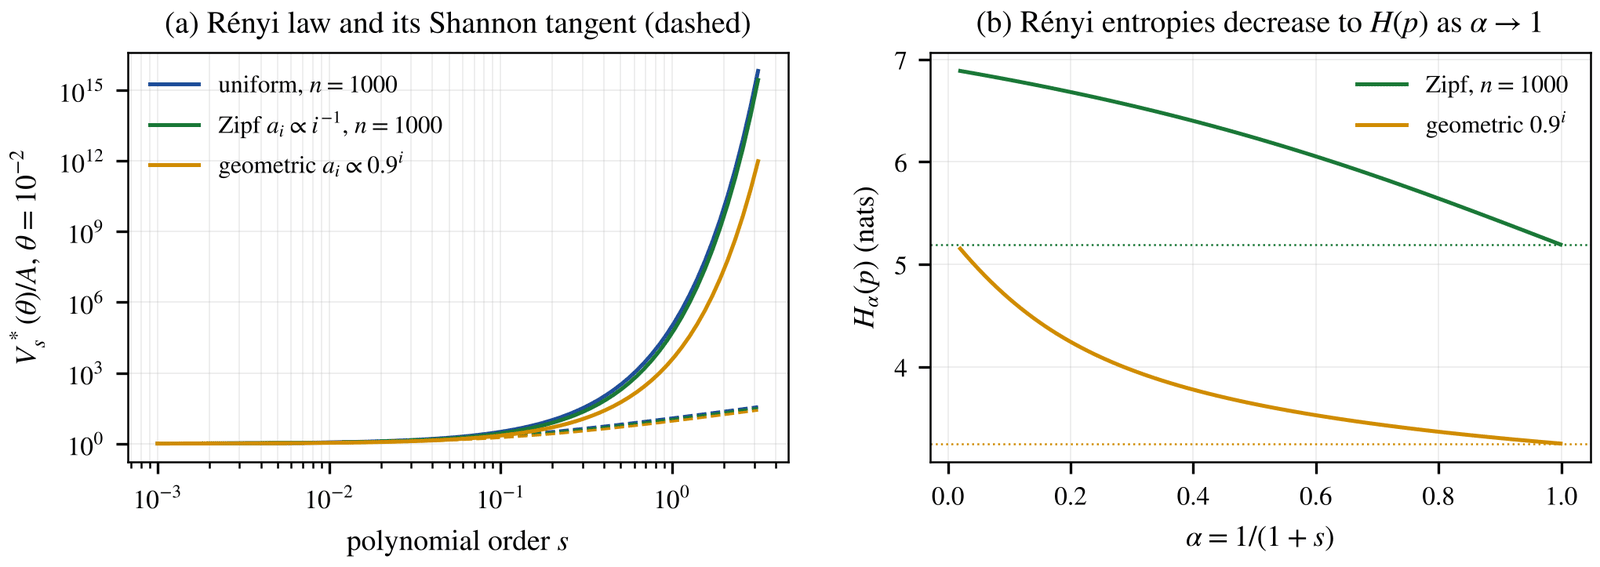
\includegraphics[width=0.98\textwidth]{figures/fig_renyi}
\caption{The R\'enyi law, Theorem~\ref{thm:D}. (a) $\Vs_{s}(\theta)/A=\theta^{-s}e^{sH_{1/(1+s)}(p)}$ at $\theta=10^{-2}$ for a uniform profile and a Zipf profile on a thousand candidates and a geometric profile of ratio $0.9$, with the Shannon tangents $1+s(H(p)+\log\frac1\theta)$ (dashed). The tangents are exact as $s\to0$ and the flat profile is the most expensive at every order. (b) The R\'enyi entropies $H_{\alpha}(p)$ of the Zipf and geometric profiles as functions of $\alpha=1/(1+s)$, decreasing to the Shannon entropy (dotted) as $\alpha\to1$.}
\label{fig:renyi}
\end{figure*}

\subsection{The duality criterion}

For infinitely many candidates the question is not the value of the optimum but whether a sound allocation of finite cost exists. The answer, for every cost function, is a single series.

Let $\kappa\colon(0,1]\to[0,\infty)$ be the cost, per unit of $a$, of making a check accept an incorrect candidate with probability at most $\delta$; so $\kappa(\delta)=\log(1/\delta)/L$ for exponential checks with a real number of runs and $\kappa(\delta)=\delta^{-s}$ for checks of order $s$. Define the \emph{dual cost}
\[
\psi(u)=\inf_{0<\delta\le1}\bigl(\kappa(\delta)+u\delta\bigr),\qquad u\ge0,
\]
the least cost of a check when each unit of false acceptance probability is charged $u$. It is the concave conjugate of $\kappa$ restricted to $(0,1]$.

\begin{theorem}[Duality criterion]\label{thm:dual}
Let $a_{n}>0$. The following are equivalent.
\begin{enumerate}[label=\textup{(\alph*)},leftmargin=2.2em,itemsep=1pt]
\item There are $\delta_{n}\in(0,1]$ with $\sum_{n}\delta_{n}<\infty$ and $\sum_{n}a_{n}\kappa(\delta_{n})<\infty$.
\item $\sum_{n}a_{n}\psi(\lambda/a_{n})<\infty$ for some $\lambda>0$.
\item $\sum_{n}a_{n}\psi(\lambda/a_{n})<\infty$ for every $\lambda>0$.
\end{enumerate}
When they hold, for every $\theta>0$ there are $\delta_{n}\in(0,1]$ with $\sum\delta_{n}\le\theta$ and $\sum a_{n}\kappa(\delta_{n})<\infty$.
\end{theorem}

\begin{proof}
(a)$\Rightarrow$(c). For every $\lambda>0$ and $n$, $0\le a_{n}\psi(\lambda/a_{n})\le a_{n}\kappa(\delta_{n})+\lambda\delta_{n}$, and the right side is summable.
(c)$\Rightarrow$(b) is trivial.
(b)$\Rightarrow$(a). By the definition of the infimum choose $\delta_{n}\in(0,1]$ with $\kappa(\delta_{n})+(\lambda/a_{n})\delta_{n}\le\psi(\lambda/a_{n})+2^{-n}/a_{n}$. Then $a_{n}\kappa(\delta_{n})+\lambda\delta_{n}\le a_{n}\psi(\lambda/a_{n})+2^{-n}$, a summable bound for two nonnegative terms, so both $\sum a_{n}\kappa(\delta_{n})$ and $\sum\delta_{n}$ converge.
For the last claim choose $N$ with $\sum_{n>N}\delta_{n}\le\theta/2$ and replace $\delta_{n}$ by $\theta/(2N)$ for $n\le N$; this changes finitely many finite terms of the cost.
\end{proof}

\begin{proposition}[The two dual costs]\label{prop:dualcosts}
\begin{enumerate}[label=\textup{(\roman*)},leftmargin=2.2em,itemsep=1pt]
\item For exponential checks, $\kappa(\delta)=\log(1/\delta)/L$, the dual is
\[
\psi(u)=\begin{cases}(1+\log(uL))/L,&uL\ge1,\\ u,&uL<1.\end{cases}
\]
\item For checks of order $s$, $\kappa(\delta)=\delta^{-s}$, the dual is
\[
\psi(u)=\begin{cases}(1+s)\,s^{-s/(1+s)}u^{s/(1+s)},&u\ge s,\\ 1+u,&u<s.\end{cases}
\]
\end{enumerate}
\end{proposition}

\begin{proof}
Both functions $\delta\mapsto\kappa(\delta)+u\delta$ are convex on $(0,1]$. In (i) the derivative $-1/(L\delta)+u$ vanishes at $\delta=1/(uL)$, which lies in $(0,1]$ exactly when $uL\ge1$, with value $\log(uL)/L+1/L$; otherwise the derivative is negative on $(0,1]$ and the minimum is at $\delta=1$. In (ii) the derivative $-s\delta^{-s-1}+u$ vanishes at $\delta=(s/u)^{1/(1+s)}$, which lies in $(0,1]$ exactly when $u\ge s$, with value $(s/u)^{-s/(1+s)}+u(s/u)^{1/(1+s)}=(1+s)s^{-s/(1+s)}u^{s/(1+s)}$; otherwise the minimum is at $\delta=1$.
\end{proof}

\begin{corollary}\label{cor:dualcases}
Let $a_{n}\to0$.
\begin{enumerate}[label=\textup{(\roman*)},leftmargin=2.2em,itemsep=1pt]
\item Exponential checks with real numbers of runs admit a sound allocation of finite cost if and only if $\sum a_{n}<\infty$ and $\sum a_{n}\log(1/a_{n})<\infty$.
\item Checks of order $s$ admit one if and only if $\sum a_{n}^{1/(1+s)}<\infty$.
\end{enumerate}
\end{corollary}

\begin{proof}
For large $n$, $u=\lambda/a_{n}$ is large, and by Proposition~\ref{prop:dualcosts} $a_{n}\psi(\lambda/a_{n})$ equals $\frac{a_{n}}L\bigl(1+\log(\lambda L)+\log\frac1{a_{n}}\bigr)$ in case (i) and a constant multiple of $a_{n}^{1/(1+s)}$ in case (ii). In case (i) the sum converges if and only if $\sum a_{n}(1+\log\frac1{a_{n}})$ does, and both terms are eventually positive. Theorem~\ref{thm:dual} concludes.
\end{proof}

The integer version needs no duality.

\begin{proposition}[Integer schedules]\label{prop:integer}
Let $0<a_{n}\le1$ with $\sum a_{n}<\infty$. There is $r\in\NN^{\NN}$ with $\sum\eps^{r_{n}}<\infty$ and $\sum a_{n}r_{n}<\infty$ if and only if $\sum a_{n}\log(1/a_{n})<\infty$; the schedule $r_{n}=\lceil\log(1/a_{n})/L\rceil$ then works, and adding $k$ runs to every check multiplies $\sum\eps^{r_{n}}$ by $\eps^{k}$.
\end{proposition}

\begin{proof}
If $r$ is such a schedule, Lemma~\ref{lem:gibbs} with $x=a_{n}$ and $y=\eps^{r_{n}}$ gives $a_{n}\log(1/a_{n})\le a_{n}r_{n}L+\eps^{r_{n}}-a_{n}\le L\,a_{n}r_{n}+\eps^{r_{n}}$, a summable bound for a nonnegative sequence. Conversely $r_{n}=\lceil\log(1/a_{n})/L\rceil$ gives $\eps^{r_{n}}\le a_{n}$ and $a_{n}r_{n}\le a_{n}\log(1/a_{n})/L+a_{n}$. The last claim is $\eps^{r_{n}+k}=\eps^{k}\eps^{r_{n}}$.
\end{proof}

Theorem~\ref{thm:dual} is the infinite form of the entropy and R\'enyi laws: it says which cost profiles can be certified at all, and Section~\ref{sec:singularity} applies it to self-improving chains.
